\documentclass{article}
\usepackage[T1]{fontenc}
\usepackage[utf8]{inputenc}
\usepackage{amsmath}
\usepackage{graphicx}
\usepackage{float}
\usepackage{listings}
\usepackage{xcolor}

\title{Explanation}
\author{Pawan Mali }
\date{June 2026}

\begin{document}
\maketitle
\section{Provided Repository structure Explanation}

I analyzed the local folder. It contains two ROS 2 workspaces:

\begin{figure}[H]
    \centering
    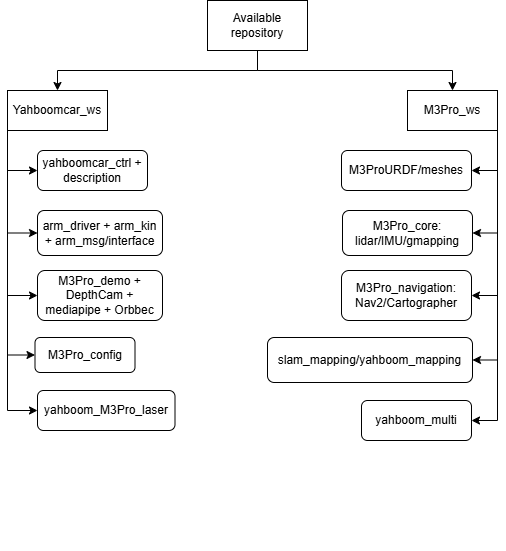
\includegraphics[width=0.9\textwidth]{Img/Repo_Downloaded.png}
    \caption{Overview of the downloaded repository structure}
    \label{fig:repo_structure}
\end{figure}

\subsection{yahboomcar\_ws/src}

\begin{itemize}
    \item \textbf{yahboomcar\_ctrl}: Keyboard and joystick teleoperation. Important files include \texttt{yahboom\_keyboard.py} and \texttt{yahboom\_joy\_M3Pro.py}.
    
    \item \textbf{yahboom\_M3Pro\_description}: Contains the robot URDF, meshes, and RViz model display files.
    
    \item \textbf{M3Pro\_config}: MoveIt2 configuration package containing arm planning settings and fake \texttt{ros2\_control} configuration.
    
    \item \textbf{M3Pro\_demo}: Includes computer vision and manipulation demonstrations such as AprilTag detection, color tracking, KCF tracking, grasping, and line-following.
    
    \item \textbf{yahboom\_M3Pro\_laser}: Lidar-based applications including obstacle avoidance, obstacle warning, and target tracking.
    
    \item \textbf{yahboom\_M3Pro\_DepthCam}: Depth camera examples including distance measurement, depth-color visualization, and edge detection.
    
    \item \textbf{OrbbecSDK\_ROS2}: ROS 2 driver package for Orbbec/Dabai depth cameras.
    
    \item \textbf{arm\_interface, arm\_msgs}: Custom messages and services used for robotic arm communication.
    
    \item \textbf{arm\_kin}: Forward and inverse kinematics services implemented using KDL.
    
    \item \textbf{arm\_driver}: Serial communication driver for the robotic arm using the Rosmaster library.
\end{itemize}

\subsection{M3Pro\_ws/src}

\begin{itemize}
    \item \textbf{M3Pro}: Robot URDF, meshes, and model display launch files.
    
    \item \textbf{M3Pro\_core}: Core robot packages including laser merging, laser filtering, IMU filtering, and GMapping support.
    
    \item \textbf{M3Pro\_navigation}: Navigation stack configuration including Nav2, Cartographer localization, and RViz navigation setups.
    
    \item \textbf{slam\_mapping, yahboom\_mapping}: Packages used for SLAM and map generation/saving.
    
    \item \textbf{ekf\_bringup}: Robot localization package that fuses \texttt{/odom\_raw} and \texttt{/imu/data} using an Extended Kalman Filter (EKF).
    
    \item \textbf{calibration}: Linear and angular calibration utilities based on \texttt{/cmd\_vel} and TF data.
    
    \item \textbf{yahboom\_multi}: Multi-robot navigation and coordination configurations.
    
    \item \textbf{patrol}: Laser-based autonomous patrol behavior implementation.
    
    \item \textbf{largemodel, largemodel\_arm}: AI, voice interaction, and computer vision application examples.
\end{itemize}
\section{Complete Hardware and software based pipeline}
\subsection{Hardware pipeline}

\begin{figure}[H]
    \centering
    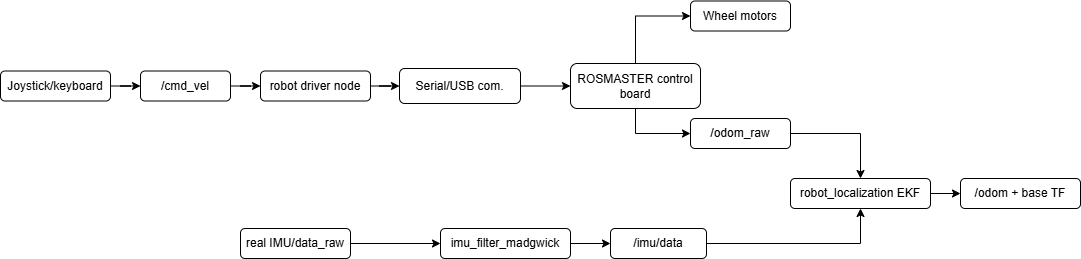
\includegraphics[width=0.9\textwidth]{Img/H_control_pipeline.png}
    \caption{Hardware control pipeline overview}
    \label{fig:H_control_pipeline}
\end{figure}

\paragraph{}

In the hardware-based system, movement commands are generated by a keyboard, joystick, and published on the \texttt{/cmd\_vel} topic. These commands are sent through the robot driver and serial communication interface to the ROSMASTER control board, which controls the motor driver and wheel motors to move the robot. Wheel encoders provide raw odometry data, while the IMU publishes motion data. The IMU data is processed using the Madgwick filter to obtain a cleaner orientation estimate. Finally, the robotlocalization EKF uses the odometry and IMU data to produce accurate robot pose information (\texttt{/odom}) transformation, which are used by RViz2, SLAM, and Nav2 for localization and navigation.


\subsection{Software pipeline}

\begin{figure}[H]
    \centering
    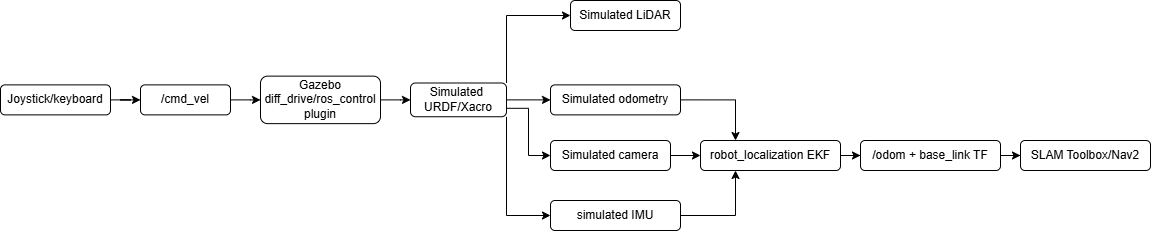
\includegraphics[width=0.9\textwidth]{Img/S_control_pipeline.png}
    \caption{Software control pipeline overview}
    \label{fig:S_control_pipeline}
\end{figure}

\paragraph{}

In the software based system, movement commands are generated by a keyboard and are published on the \texttt{/cmd\_vel} topic. Instead of being sent to a physical robot, these commands are processed by a Gazebo \texttt{diff\_drive} or \texttt{ros2\_control} plugin, which moves the simulated robot model defined by the URDF/Xacro files. As the robot moves within the virtual environment, Gazebo generates simulated sensor data, including odometry, IMU, LiDAR, and camera information. The odometry and IMU data are used by the \texttt{robot\_localization} Extended Kalman Filter (EKF) to produce accurate robot pose estimates and the \texttt{odom} to \texttt{base\_link} transformation. The simulated LiDAR data is used by SLAM Toolbox and Nav2 for mapping, localization, and path planning, while the simulated camera data can be utilized for computer vision tasks such as object detection and obstacle avoidance. This simulation-based architecture enables the development, testing, and validation of robotic algorithms without requiring physical hardware.

\section{Task 1: Simulation based teleoperation}
For this first step, the pipeline contains only:
\begin{itemize}
\item M3Pro base model
\item Gazebo physics
\item robot state publisher
\item Keyboard or joystick teleoperation
\item cmd vel
\item Gazebo movement plugin
\end{itemize}

\subsection{keyboard teleoperation}

\textbf{Previous hardware pipeline:}

\begin{figure}[H]
    \centering
    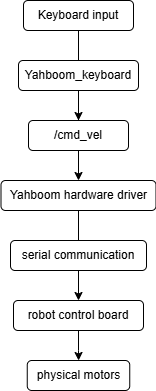
\includegraphics[width=0.25\textwidth]{Img/Keyboard Hardware pipeline.png}
    \caption{Hardware pipeline overview}
    \label{fig:H_control_pipeline}
\end{figure}

The existing \texttt{yahboomcar\_keyboard.py} node can be used without any changes.

\textbf{New software pipeline:}

\begin{figure}[H]
    \centering
    \includegraphics[width=0.25\textwidth]{Img/Keyboard software pipeline.png}
    \caption{Software pipeline overview}
    \label{fig:S_control_pipeline}
\end{figure}

\section{understand the repo structure and debug the errors}
What's actually in this repo
    \begin{itemize}
    \item Two workspaces: {yahboomcar\_ws} (arm driver, robot description/URDF, MoveIt2 config, laser, depth camera) and {M3Pro\_ws} (navigation2, SLAM, calibration, and a big ``largemodel'' AI/voice stack).
    \item The {Docker\_M3Pro-*.sh} scripts pull an image from 192.168.2.51:5000 --- that's a private LAN registry inside Yahboom's factory network, not reachable from your our system at all.
    \item Hardware drivers are hardcoded, e.g. {arm\_driver.py} does {Rosmaster("/dev/ttyUSB0")} using a proprietary \texttt{Rosmaster\_Lib} pip package. Without hardware, this will throw \texttt{SerialException: could not open port /dev/ttyUSB0}.
    \item The only working "no-hardware" launch files are plain URDF viewers (display.launch.py), which just start robot\_state\_publisher + joint\_state\_publisher.

\end{itemize}

\subsection{RViz2 / Robot Description Debugging}
During comiling the repo, I encountered some errors related to missing packages and dependencies. To resolve these issues, I followed these steps:

\begin{figure}[H]
    \centering
    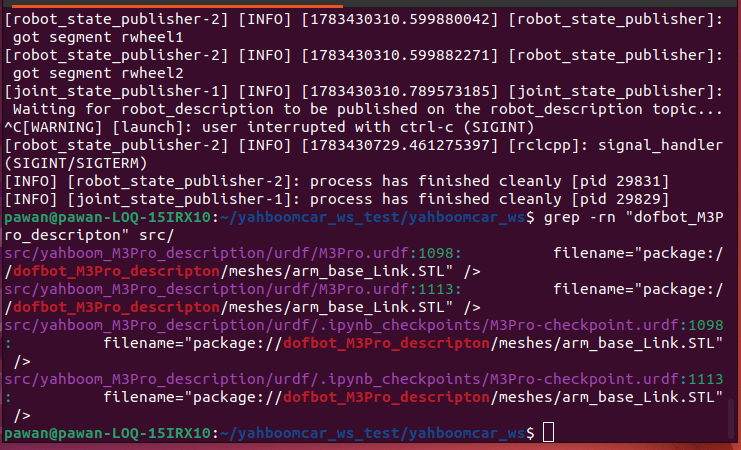
\includegraphics[width=0.8\textwidth]{Img/urdf.png}
    \caption{URDF errors}
    \label{fig:URDF_errors}
\end{figure}
The robot model initially showed an error because the package name in the URDF file was incorrect. The error was found at lines 1098 and 1113. According to the correction, rebuilt the workspace using colcon build, and launched the model again. After the correction, the robot appeared successfully without errors.

\subsection{RViz2 / Controlling the Robot movement}

I tested the Chassis Control Course, especially section 3.3.1 - Controlling the Car’s Speed, without connecting the real robot hardware.


After launching the robot description using display.launch.py. The URDF model loaded correctly in RViz, and the robot was visible without errors. I then checked the active ROS 2 nodes and topics. Only visualization-related nodes such as robot state publisher, joint state publisher, and RViz were running. There was no chassis driver or motor control node.

\begin{figure}[H]
    \centering
    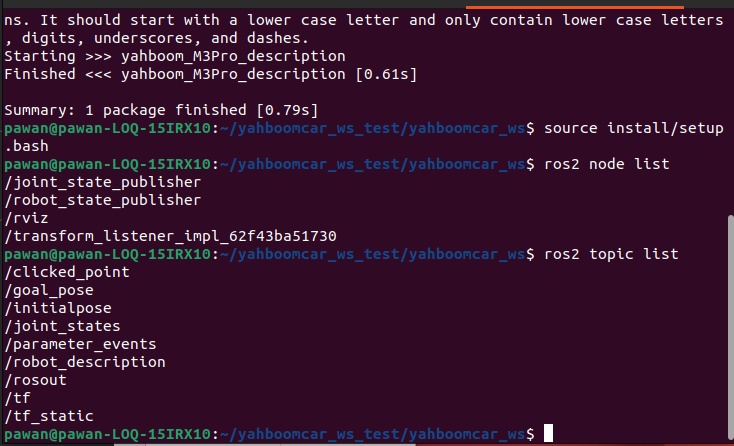
\includegraphics[width=1\textwidth]{Img/topiclist.png}
    \caption{Node and Topic List}
    \label{fig:node and topic list}
\end{figure}


Next, a velocity command was published to the \texttt{/cmd\_vel} topic:

\begin{lstlisting}[language=bash, basicstyle=\ttfamily\small, breaklines=true]
ros2 topic pub /cmd_vel geometry_msgs/msg/Twist \
"{linear: {x: 0.1, y: 0.0, z: 0.0}, angular: {x: 0.0, y: 0.0, z: 0.0}}" --once
\end{lstlisting}

The command continuously showed:

\begin{lstlisting}[basicstyle=\ttfamily\small, breaklines=true]
Waiting for at least 1 matching subscription(s)...
\end{lstlisting}

This happened because no node was subscribed to \texttt{/cmd\_vel}. On the real robot, the chassis driver receives this command, sends motor speed values to the STM32 controller through serial communication, reads encoder data, and publishes odometry. Since the hardware and chassis driver were not available, the velocity command had no receiver.

\begin{figure}[H]
    \centering
    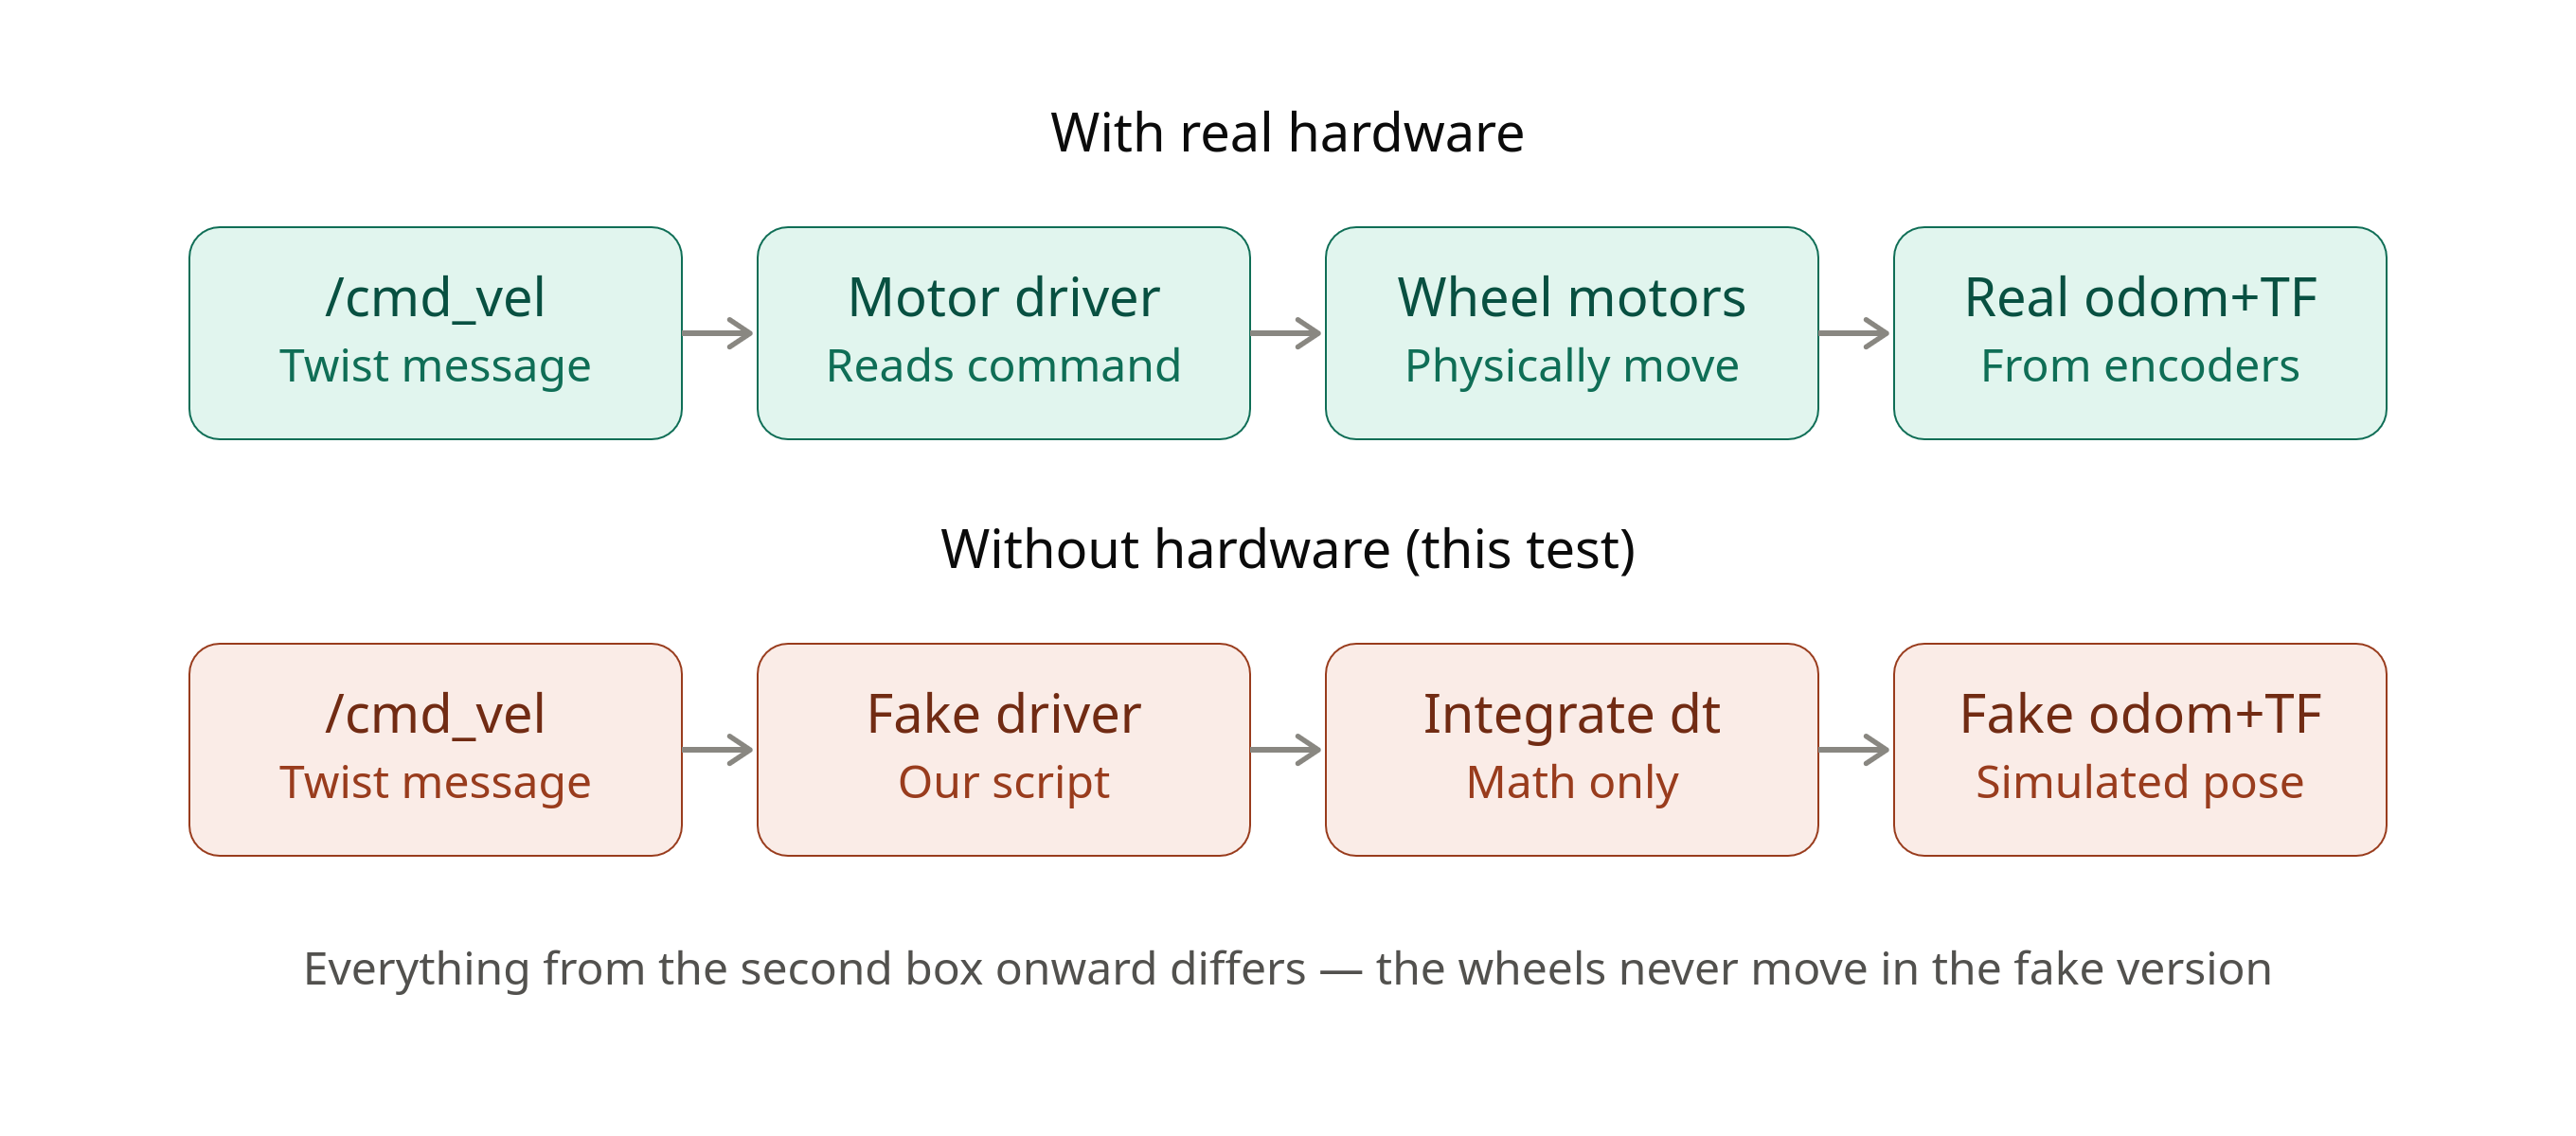
\includegraphics[width=1\textwidth]{Img/real_vs_fake_control_pipeline.png}
    \caption{Real vs. Fake Control Pipeline}
    \label{fig:real_vs_fake_control_pipeline}
\end{figure}

To test the chassis-control command without the real robot hardware, a temporary node called \texttt{fake\_odom\_driver.py} was added. The original command publishes velocity values on \texttt{/cmd\_vel}, but no real motor driver is available to receive them. Therefore, the robot cannot move in RViz using only \texttt{robot\_state\_publisher}.

The fake driver works as a simple software replacement for the hardware driver. It subscribes to \texttt{/cmd\_vel} and reads the commanded forward, sideways, and rotational velocities. These values are stored as:

\begin{lstlisting}[basicstyle=\ttfamily\small, breaklines=true]
linear.x  -> forward/backward movement
linear.y  -> sideways movement for mecanum wheels
angular.z -> rotation
\end{lstlisting}

The node then calculates the robot's new position over time using simple dead-reckoning. It updates the robot's \(x\), \(y\), and heading angle based on the latest velocity command. After calculating the pose, it publishes an odometry message on \texttt{/odom} and broadcasts the TF transformation:

\begin{lstlisting}[basicstyle=\ttfamily\small, breaklines=true]
odom -> base_link
\end{lstlisting}

RViz uses this TF transformation to update the position of the complete robot model. The robot links and joints are still displayed by \texttt{robot\_state\_publisher}, while the fake driver changes the position of the robot base.

\subsection{Set Gazebo Environment / Control the Robot movement}

```latex
\subsection{Base Movement Control in Gazebo Simulation}

\subsubsection{Objective}

The objective of this stage was to make the ROSMASTER M3Pro mobile base movable and controllable in Gazebo Classic using a holonomic control method suitable for its mecanum-wheel configuration. The simulated robot should be capable of forward and backward motion, lateral movement, and rotation around its vertical axis.

\subsubsection{Control Approach}

The mobile base was controlled using the Gazebo Classic \texttt{libgazebo\_ros\_planar\_move.so} plugin. This plugin subscribes to the \texttt{/cmd\_vel} topic and directly applies linear and angular velocities to the robot chassis.

The planar movement plugin supports velocity commands in the longitudinal direction, lateral direction, and yaw rotation. Therefore, the robot can perform holonomic movements such as sideways strafing, which is suitable for a mecanum-wheeled mobile platform.

In this initial simulation approach, the individual wheel-contact kinematics and mecanum roller dynamics are not modelled. Instead, the commanded chassis velocity is applied directly to the robot base. This provides a simple and reliable method for validating keyboard control, navigation commands, odometry, and the overall simulation architecture.

\subsubsection{Files Added}

The following Xacro files were added to the robot description package:

\begin{itemize}
    \item \texttt{urdf/M3Pro.planar\_move.xacro}

    This file defines the \texttt{M3Pro\_gazebo\_planar\_move} macro. The macro contains the Gazebo planar movement plugin configuration, including the command velocity topic, odometry topic, odometry frame, robot base frame, and odometry publishing settings.

    \item \texttt{urdf/M3Pro.wheel\_friction.xacro}

    This file defines the \texttt{M3Pro\_wheel\_friction} macro. It configures the Gazebo friction parameters \texttt{mu1} and \texttt{mu2} for all four wheels. The friction coefficients were reduced to near-zero values because the wheels are not used to physically generate the robot motion when the planar movement plugin is active.
\end{itemize}

\subsubsection{Files Modified}

The following existing files were modified:

\begin{itemize}
    \item \texttt{urdf/M3Pro.urdf.xacro}

    The planar movement and wheel-friction Xacro files were included in the main robot description. Their corresponding macros were then called so that the plugin and friction parameters became part of the robot model loaded into Gazebo.

    \item \texttt{launch/gazebo\_display.launch.py}

    A \texttt{joint\_state\_publisher} node was added to publish joint states for non-driven joints, including the wheel and camera joints. This allowed RViz2 to resolve and display the complete TF tree of the robot.
\end{itemize}

\subsubsection{Implementation and Testing}

After integrating the planar movement plugin, the robot was tested by publishing velocity commands directly to the \texttt{/cmd\_vel} topic. The following types of movement were successfully verified:

\begin{itemize}
    \item Forward and backward movement using the linear velocity component \texttt{linear.x}.
    \item Sideways strafing using the lateral velocity component \texttt{linear.y}.
    \item Clockwise and counter-clockwise rotation using the angular velocity component \texttt{angular.z}.
\end{itemize}

An example command used to test forward movement is shown below:

\begin{verbatim}
ros2 topic pub /cmd_vel geometry_msgs/msg/Twist \
"{linear: {x: 0.3, y: 0.0, z: 0.0},
  angular: {x: 0.0, y: 0.0, z: 0.0}}"
\end{verbatim}

Similarly, lateral movement was tested by assigning a non-zero value to \texttt{linear.y}, while rotational movement was tested by assigning a non-zero value to \texttt{angular.z}.


\subsubsection{Wheel Joint Type and Limit Configuration}

The M3Pro drive wheels must be able to rotate continuously during forward, backward, lateral, and rotational motion. Therefore, the wheel joints should be defined as \texttt{continuous} joints rather than \texttt{revolute} joints.

A \texttt{revolute} joint requires lower and upper angular limits. For example:

\begin{verbatim}
<joint name="wheel_joint" type="revolute">
    <limit lower="-1.0"
           upper="1.0"
           effort="100"
           velocity="100"/>
</joint>
\end{verbatim}

In this configuration, the wheel can rotate only between $-1$ radian and $+1$ radian. This corresponds to a total angular range of:

\[
2~\text{rad} \approx 114.6^\circ
\]

Therefore, the wheel can rotate only approximately one-third of a complete revolution before reaching its position limit. Once the joint reaches either the lower or upper limit, Gazebo prevents any further rotation. Although the velocity limit is set to \texttt{100 rad/s}, this does not remove the angular position restriction.

For this reason, a \texttt{revolute} joint is more suitable for limited-motion joints such as robot arm joints, steering joints, gripper joints, or camera tilt joints.

For the M3Pro drive wheels, the correct configuration is:

\begin{verbatim}
<joint name="wheel_joint" type="continuous">
    <limit effort="10"
           velocity="10"/>
</joint>
\end{verbatim}

A \texttt{continuous} joint can rotate indefinitely in both directions. Therefore, the \texttt{lower} and \texttt{upper} position limits are not required.

The \texttt{effort} parameter defines the maximum torque that may be applied to the joint, while the \texttt{velocity} parameter defines the maximum permitted angular velocity. In this simulation, setting both parameters to non-zero values allowed the wheel joints to move freely when the planar movement plugin commanded the robot chassis.

The previous wheel joint configuration used:

\begin{verbatim}
<limit lower="0"
       upper="0"
       effort="0"
       velocity="0"/>
\end{verbatim}

This configuration did not permit useful wheel motion. The zero velocity limit prevented wheel rotation, while the zero effort limit did not allow torque to be applied to the joint. In addition, the identical lower and upper limits represented a fixed angular position.

After changing the wheel joints to \texttt{continuous} joints and using:

\begin{verbatim}
<limit effort="10"
       velocity="10"/>
\end{verbatim}

the wheels were able to rotate without angular restrictions. This eliminated the abnormal wheel resistance observed during chassis movement and helped resolve the Gazebo tipping behaviour.


\subsubsection{Result}

The M3Pro mobile base is fully functional in the Gazebo Classic simulation. Forward movement, backward movement, lateral strafing, and rotation were successfully tested. The wheel-friction modification eliminated the chassis-tipping problem, while the planar movement plugin provided stable holonomic motion.

The simulated odometry and TF data were also verified using ROS~2 command-line tools and RViz2. Therefore, the base movement stage provides a functional foundation for the subsequent integration of keyboard teleoperation, SLAM, localization, obstacle avoidance, and Nav2-based autonomous navigation.


\end{document}

